\section{Auswertung und Diskussion}
In den Abbildungen \ref{fig:bwsx}, \ref{fig:bwsy} und \ref{fig:bwsz} ist die Dosisverteilung in der
Brustwirbelsäule in der Transversal-, Sagittal- und Frontalansicht gezeigt. In den Abbildungen ist zu erkennen, dass die $\SI{95}{\percent}$
Isodosenlinie das rot eingezeichnete PTV in den meisten Bereichen vollständig umschließt. Allerdings ist es nicht überall gelungen eine relative Dosis von
$95\%$ zu erreichen. Das kommt daher, da das Zielvolumen sehr groß ist und deshalb von unterschiedlichen Gewebe umgeben ist.
Aus diesem Grund ist es sehr schwierig in dem PTV eine homogene Dosisverteilung zu erreichen. Für eine bessere Beurteilung ist das
Dosis-Volumen-Histogramm in der Abbildung \ref{fig:bwsdvh} gezeigt. Anhand der DVH Kurve für das PTV (rot) ist zu erkennen, dass
lediglich in einem kleinen Teil des PTVs es nicht gelungen ist eine Dosis von $\SI{95}{\percent}$ zu erreichen, denn
noch etwa $94\%$ des PTVs erhält $95\%$ der Dosis.
Die minimale Dosis, die im PTV deponiert wird liegt bei  $\SI{86.5}{\percent}$ Isodosenlinie, also unterhalb der gewünschten $95\%$, was auch schon
anhand der Dosisverteilung gesehen werden konnte.
Ein weiterer Grund, dass das PTV nicht komplett mit der $95\%$ Isodosenlinie umschlossen werden konnte ist, dass
die umliegenden Risikoorgane so gut wie möglich geschont werden müssen.

\begin{figure}[H]
	\centering
	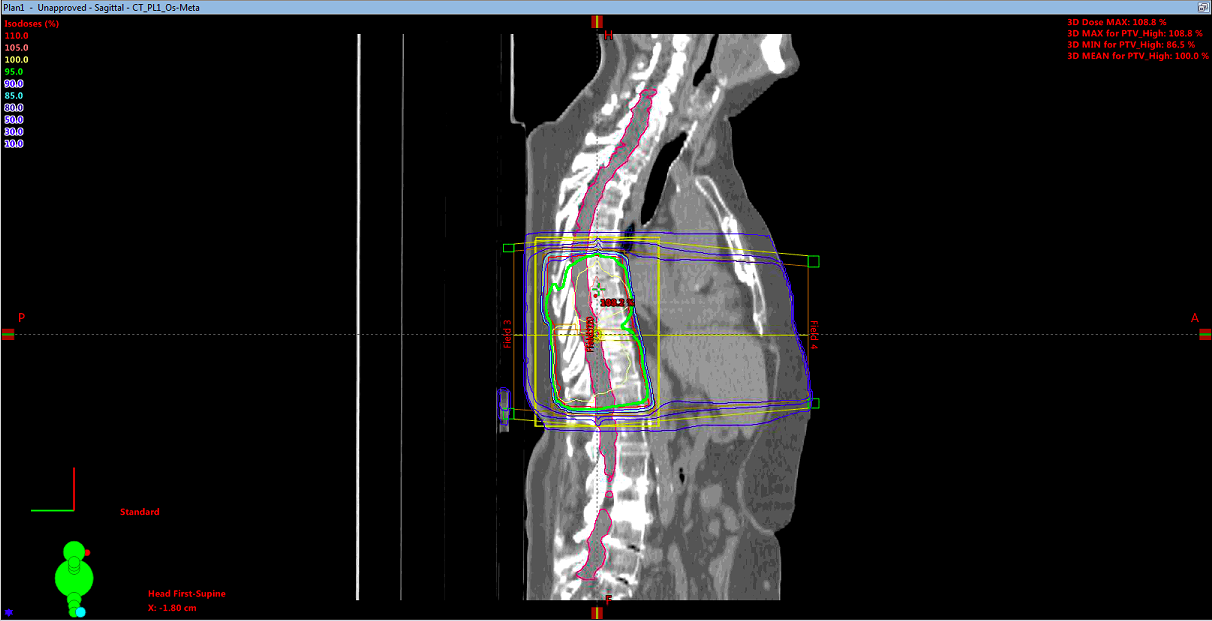
\includegraphics[width=\linewidth]{Bilder/BWS_X}
	\caption{Darstellung der Dosisverteilung in der Sagittalansicht des Oberkörpers.}
	\label{fig:bwsx}
\end{figure}

\begin{figure}[H]
	\centering
	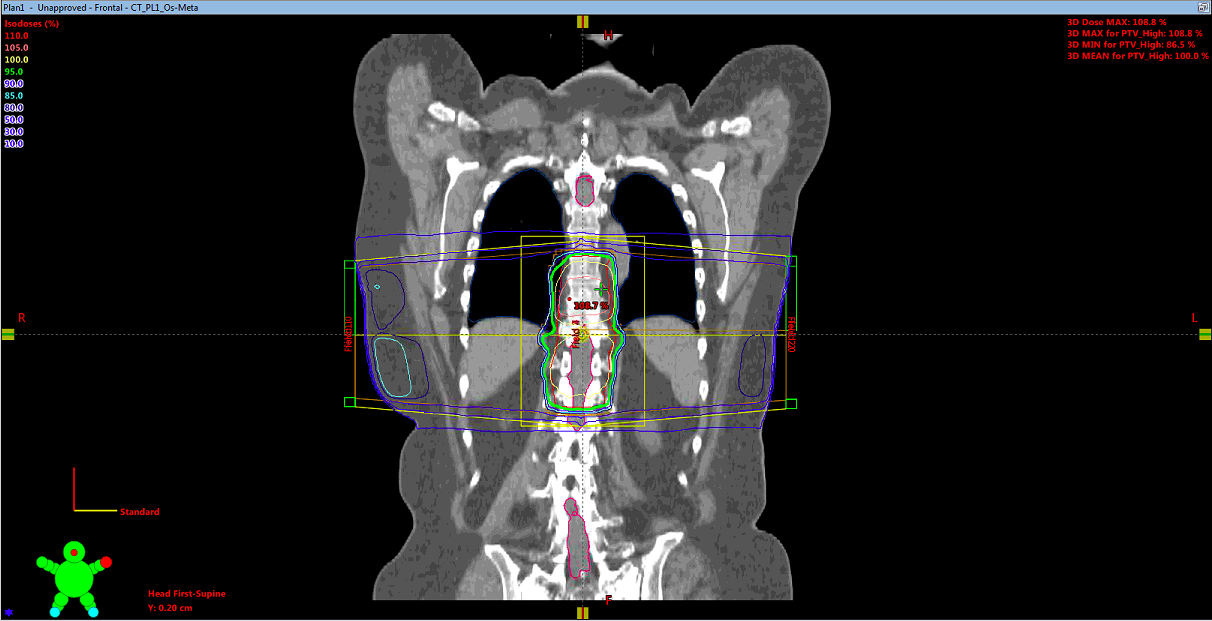
\includegraphics[width=\linewidth]{Bilder/BWS_Y}
	\caption{Darstellung der Dosisverteilung in der Frontalansicht des Oberkörpers.}
	\label{fig:bwsy}
\end{figure}

\begin{figure}[H]
	\centering
	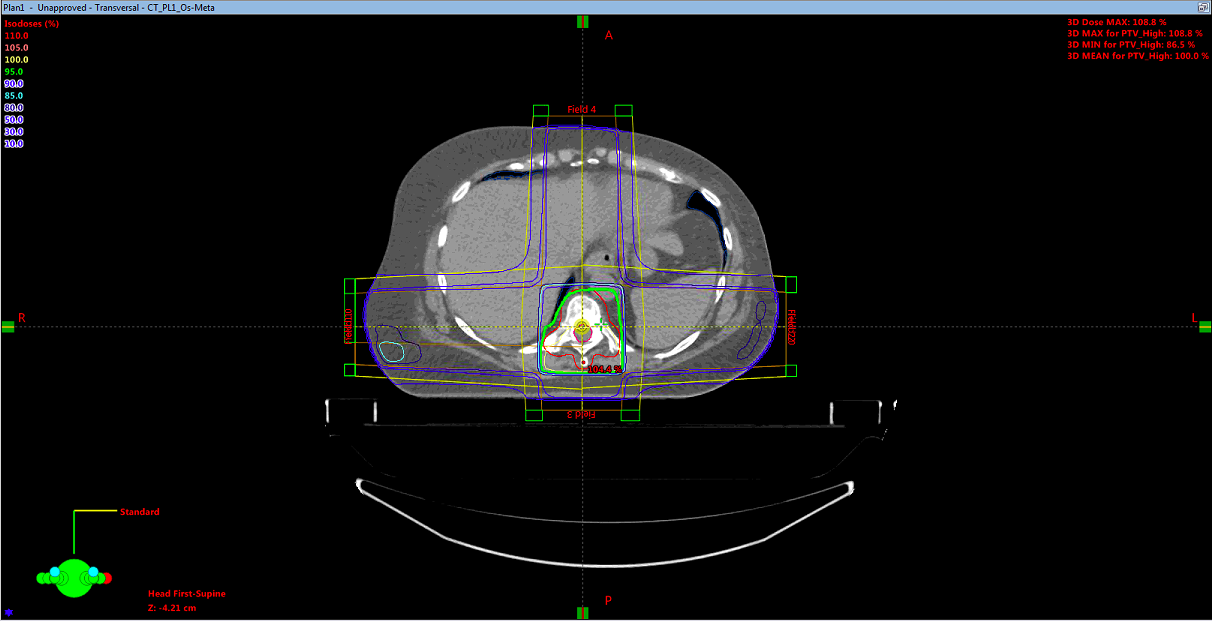
\includegraphics[width=\linewidth]{Bilder/BWS_Z}
	\caption{Darstellung der Dosisverteilung in der Transversalansicht des Oberkörpers.}
	\label{fig:bwsz}
\end{figure}

Die maximale relative Dosis $\SI{108,8}{\percent}$ wird in dem PTV deponiert und überschreitet die erlaubte maximale
Dosis von $\SI{107}{\percent}$ nur minimal und anhand des DVHs kann gesehen werden, dass in einem sehr kleinen Teil des PTVs
diese hohe Dosis deponiert wird \cite{ICRU}.
Anhand des DVHs des gesamten Thorax (grüne Kurve) ist zu erkennen, dass in dem gesamten Thorax nur eine relativ geringe Dosis deponiert wird.
Etwa $\SI{11}{\percent}$ des Thoraxvolumens erhält eine Dosis von  $\SI{50}{\percent}$. Durch die DVH Kurven der Risikoorgane ist zu erkennen,
dass sie zum Teil gut geschont werden konnten. Von den Risikoorganen erhält das Rückenmark die meiste Dosis, was bei der Lokalisation des Zielvolumens
zu erwarten war.\\
Es muss noch überprüft werden, ob die Organdosisgrenzwerte eingehalten worden sind.
Die mittlere Dosis der Lunge darf $\SI{20}{\gray}$ nicht überschreiten
und es darf nicht mehr als $\SI{30}{\percent}$ des Lungenvolumens eine Dosis von $\SI{20}{\gray}$ erhalten \cite{grenz}.
Diese Grenzwerte wurden erfolgreich eingehalten, weil nur $\SI{18,58}{\percent}$ des Volumens der gesamten Lunge eine
Dosis von $\SI{20}{\gray}$ erhält und die mittlere Dosis liegt bei $\SI{7,659}{\gray}$.
Der rechte Lungenflügel erhält eine mittlere Dosis von $\SI{8,24}{\gray}$ und der linke Lungenflügel eine mittlere Dosis von $\SI{6,84}{\gray}$.
Die mittleren Dosen der beiden Lungenflügel liegen auch unter dem $\SI{20}{\gray}$ Wert und auch die beiden Lungenvolumen liegen unter dem Grenzwert.
Bei der rechten Lungenflügel ergibt sich bei einer Dosis von $\SI{20}{\gray}$ in $\SI{19,37}{\percent}$ des Volumens und bei dem linken
Flügel in $\SI{17,43}{\percent}$ des Volumens.
Der Grenzwert für die mittlere Dosis
für das Herz beträgt $\SI{26}{\gray}$ und weniger als $\SI{46}{\percent}$ des Herzvolumens darf eine Dosis von $\SI{30}{\gray}$ erhalten \cite{grenz}.
Dies wurde auch erfolgreich eingehalten, da $\SI{1,22}{\percent}$ des Volumens mit einer Dosis von $\SI{30}{\gray}$ bestrahlt wird und die mittlere
Dosis liegt bei $\SI{14,761}{\gray}$.
Bei dem Rückenmark darf die maximale Dosis $\SI{45}{\gray}$ nicht überschreiten \cite{grenz}.
Allerdings wird bei dieser Therapie mit einer Gesamtdosis von $\SI{45}{\gray}$ bestrahlt und
da das Rückenmark durch das PTV verläuft ist es unmöglich unterhalb von den Grenzwert zu bleiben.
Bei diesem Plan liegt die maximale Dosis des Rückenmarks bei $\SI{48.94}{\gray}$.
Der Grenzwert $\SI{45}{\gray}$ ist ein Wert, der von dem Klinikum Dortmund festgelegt worden ist und dabei
handelt es sich um einen sehr konservativen Grenzwert. Der Grenzwert für das Rückenmark, nach der QUANTEC Tabelle, liegt für
die maximale Dosis bei $\SI{50}{\gray}$ \cite{QUANTEC}. Dieser Wert konnte mit diesem Bestrahlungsplan eingehalten werden und deshalb
ist die hohe maximale Dosis des Rückenmarks akzeptabel.
Bei der Niere darf die mittlere Dosis $\SI{15}{\gray}$ bis $\SI{18}{\gray}$ nicht überschreiten \cite{grenz}.
Auch diese Werte wurden erfolgreich eingehalten, da
bei der linken Niere die mittlere Dosis $\SI{6,433}{\gray}$ beträgt und bei der rechten $\SI{4,022}{\gray}$.
Die mittlere Dosis der Leber liegt bei $\SI{11,455}{\gray}$. Auch bei der Leber wurde der Grenzwert eingehalten,
da der Obergrenzwert der mittleren Dosis der Leber bei $\SI{30}{\gray}$ bis $\SI{32}{\gray}$ liegt \cite{QUANTEC}.

\begin{figure}[H]
	\centering
	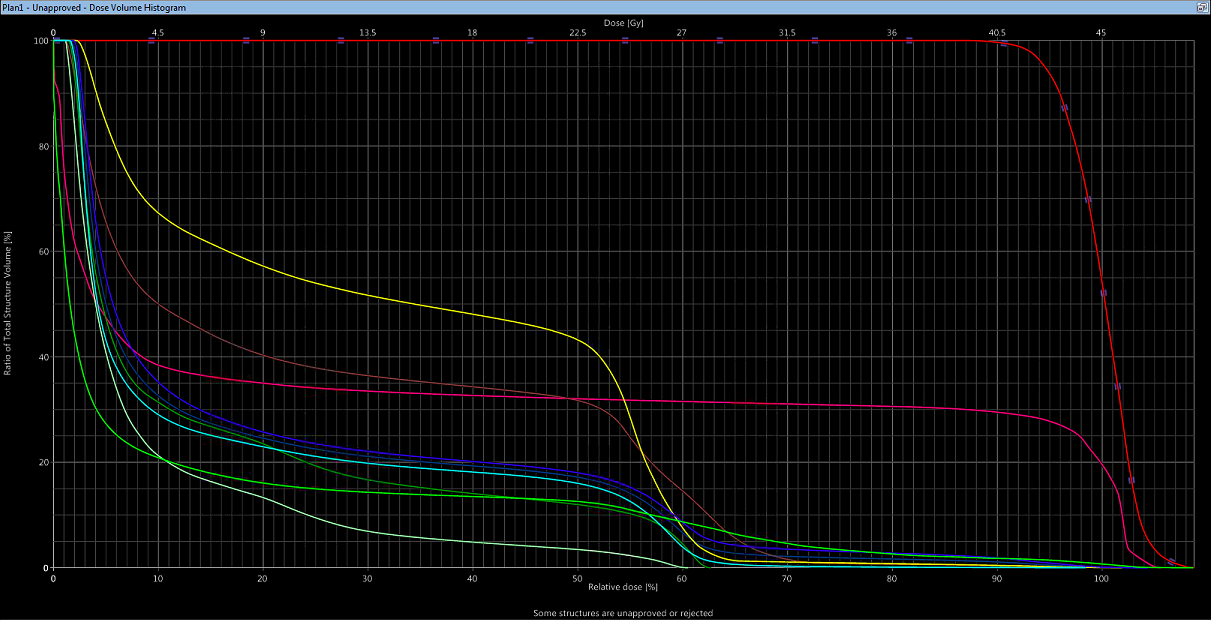
\includegraphics[width=\linewidth]{Bilder/BWS_DVH}
	\caption{Zu sehen ist das Dosis-Volumen-Histogramm. In roter Farbe dargestellt ist das PTV-High und in grüner Farbe ist der gesamte Thorax. Außerdem sind noch die einzelnen Isodosenlinien eingezeichnet und die einzelnen Kurven zu den Risikoorgane wie z.B. Herz (gelb), Leber (braun), Lunge rechts (hellblau), Lunge links (blau), Lunge gesamt (dunkelblau), Niere rechts (hellgrün), Niere links(dunkelgrün) und das Rückenmark(pink).}
	\label{fig:bwsdvh}
\end{figure}

Bei dem erstellten Plan konnte nicht erreicht werden, dass das PTV komplett von der $\SI{95}{\percent}$
Isodosenlinie umschlossen wird. Das liegt daran, da das Zielvolumen, wie in den Abbildungen \ref{fig:bwsx}, \ref{fig:bwsy} und \ref{fig:bwsz}
zu sehen, sehr groß ist. Außerdem befinden sich viele Risikoorgane in unmittelbarer Nähe zu dem Zielvolumen.
Da durch die verwendeten Felder, mit individuell angepassten MLCs, die Organdosisgrenzwerte fast aller Risikoorgane eingehalten werden konnten,
kann mit diesem Plan eine adäquate Behandlung gewährleistet werden.
